\documentclass{article}

% NeurIPS 2026 style. "preprint" = non-anonymous, no line numbers, footer "Preprint."
% (not "final", whose footer would claim the paper appeared at NeurIPS 2026).
\PassOptionsToPackage{numbers,sort&compress}{natbib}
\usepackage[preprint]{neurips_2026}
\usepackage{graphicx}
\usepackage[utf8]{inputenc}
\usepackage[T1]{fontenc}
\usepackage{hyperref}
\usepackage{url}
\usepackage{booktabs}
\usepackage{amsmath,amsfonts}
\usepackage{microtype}
\usepackage{xcolor}

% Draft markers: every \TBD{} must be gone before submission.
\newcommand{\TBD}[1]{\textcolor{red}{[#1]}}
\newcommand{\ours}{concept pruning}

\title{NLP final project}

\author{Or Davidovich\\Technion -- Israel Institute of Technology}

\begin{document}
\maketitle

\begin{abstract}
In the embedding baselines of the MulTaBench text–tabular benchmark, each free-text column is embedded, compressed with PCA, and given to a tree model together with the table; Joint TAR also fine-tunes the text encoder on the target. We ask how the
target can be used further on top of TAR. Our first approach \emph{removes} information: a sparse autoencoder (SAE)
splits each column's embeddings into concepts, each concept is tested against a shuffled copy of itself inside one
model with the table, and the concepts that fail are subtracted before compression. On the 20
text datasets of MulTaBench this selection is far better than removing random concepts of the same total variance
(16/20 datasets, $p<0.001$), but does not improve on TAR, even when the amount removed is chosen by nested
cross-fitting. Reweighting the embedding or re-learning its compression (PLS, no compression, a trained 30-unit
bottleneck) does not help either. What helps is \emph{adding}: the out-of-fold predictions of a text-only model, stacked as extra columns next
to TAR's, improve on TAR with tuned LightGBM ($+0.0035$, 16/20, Holm-adjusted $p=0.007$) and with CatBoost
($+0.0036$, 17/20, $p=0.004$). With default LightGBM it wins on 15/20 datasets but is not significant ($p=0.064$): its mean is pulled below zero by two folds of one 114-class dataset on which the default learner collapses. Code: \url{https://github.com/fireflyOr/NLP-final-project}
\end{abstract}

% ------------------------------------------------------------------------------------------------------------
\section{Introduction}

Many tabular datasets contain free-text columns next to numerical and categorical ones, such as the description of a job posting or the text of a product review. A standard pipeline embeds each text cell with a pretrained encoder, reduces it to a few dimensions, and gives the result to a
gradient-boosted tree model alongside the other columns \citep{shi2021multimodal,grinsztajn2022tree}. 
Among its baselines, MulTaBench
\citep{multabench} includes two such pipelines: Joint Frozen embeds each text column with a frozen E5-small encoder \citep{wang2022e5} and keeps 30 principal components per column; Joint TAR first fine-tunes the encoder on the target, with the aim of making the embeddings, and therefore the components, target-aware.

Both pipelines compress each column to 30 dimensions, and PCA decides what survives by variance, not by
relevance. Fine-tuning shifts the embedding toward the target, but it does not control the compression: if a frequent
but irrelevant theme, like shipping or brand tone, varies more than the price-relevant content of a product description,
it still takes up the components. Our goal is therefore to remove target-irrelevant content \emph{before}
compressing, so that what PCA discards is the least relevant part. Sparse autoencoders (SAEs) make this possible by
writing an embedding as a sparse combination of learned, often interpretable directions
\citep{bricken2023monosemanticity,cunningham2023sparse,gao2024scaling}. We use them as a filter, and compare removal
with two other ways of using the target on top of TAR: reweighting the embedding, and adding a text model's
prediction. Our contributions are: (i)~SAE concept pruning for text-tabular pipelines, with a joint shadow
test of every concept and a nested cross-fit variant (\S\ref{sec:method}); (ii)~a paired leakage-controlled
evaluation on all 20 MulTaBench text datasets with three learners, in which every arm of a fold uses the same saved
TAR fine-tune (\S\ref{sec:setup}); and (iii)~the finding that removal and reweighting do not improve on TAR while
adding does: out-of-fold text stacking on TAR is significantly better than TAR with tuned LightGBM and with CatBoost
(\S\ref{sec:results}).

% ------------------------------------------------------------------------------------------------------------
\section{Related work}

Tree ensembles over compressed text embeddings are strong text--tabular baselines
\citep{shi2021multimodal,multabench}; Joint TAR makes the embeddings target-aware by fine-tuning the encoder
\citep{multabench}, and tabular foundation models such as TabSTAR \citep{arazi2025tabstar} do so inside the model.
Our three uses of the target build on established ideas. \emph{Removing} is feature selection:
marginal importance is unreliable for redundant features \citep{strobl2008conditional}, so Boruta
\citep{kursa2010boruta} compares each feature with permuted ``shadow'' copies inside one model; our features are the
concepts of TopK SAEs \citep{gao2024scaling}, a tool from mechanistic interpretability
\citep{bricken2023monosemanticity,cunningham2023sparse}. \emph{Reweighting} follows supervised PCA
\citep{bair2006prediction} and PLS \citep{wold2001pls}, which use the target to choose components. \emph{Adding}
follows stacked generalization \citep{wolpert1992stacked}: out-of-fold predictions feed a second learner, as in
cross-fitting \citep{chernozhukov2018double}.
% ------------------------------------------------------------------------------------------------------------
\section{Method}\label{sec:method}

\paragraph{Pipeline.} For each text column $c$, $x\in\mathbb{R}^{384}$ is the (frozen or TAR-tuned) E5 embedding of
``\texttt{passage: $c$: value}''. Joint Frozen and Joint TAR fit PCA-30 on the training rows and pass it to the tree model together with the table. Every method below is fitted on the training rows only.

\paragraph{Removing: concept pruning.} We train a TopK SAE \citep{gao2024scaling} on the column's training
embeddings, without labels. Its encoder maps $x$ to 2048 non-negative activations and keeps only the $k=32$ largest
($z\in\mathbb{R}^{2048}$, at most 32 non-zero); its decoder reconstructs $\hat x = b + \sum_i z_i d_i$, where each
$d_i$ is a unit-norm direction and $b$ a bias. We call each latent $i$, with direction $d_i$ and activation $z_i$, a
\emph{concept}. The SAE leaves on average 2\% of the variance unexplained. Concepts active on fewer than 20 training rows are too rare to
test and are always kept.
We ask, for each concept, whether the target-prediction model uses it
more than it would use a meaningless copy of it (a group variant of Boruta \citep{kursa2010boruta}), in four steps.
(i)~\emph{Sibling groups.} Concepts whose decoder directions are nearly identical (average-linkage cosine distance
below 0.5) are grouped and treated as one unit; otherwise two concepts that duplicate each other could each look
unnecessary and both be removed. (ii)~\emph{Shadows.} For each group we add a \emph{shadow}: the group's activations
with the rows shuffled. It has the same values and sparsity as the real group but no relation to the target, so it
shows how much a group can seem useful by chance. (iii)~\emph{One joint model.} A single LightGBM predicts the target
from the table, all concepts, and all shadows (200 trees, 30\% of the columns per tree so that every concept gets
chances to be used). Fitting them together means a concept that only repeats a table column, or helps only together
with other concepts, is judged in that context. A group's \emph{gain} is the total reduction in training loss
achieved by the splits that use its concepts. (iv)~\emph{Decision.} A group is kept if its gain exceeds its own
shadow's gain in at least two of three repetitions with fresh shuffles, and removed otherwise.

The removed concepts $\mathcal{D}$ are subtracted from the embedding, $\tilde x = x-\sum_{i\in\mathcal{D}} z_i d_i$.
Subtracting, rather than rebuilding $x$ from the kept concepts, leaves everything else in $x$ unchanged, including
the small part the SAE does not reconstruct. PCA-30 is then fitted on $\tilde x$, so the learner receives the same
number of text features as with Joint Frozen and Joint TAR.




\emph{Cross-fitted variant.} TAR has partly memorized its training rows, so on them many concepts can look
useful. This variant decides \emph{how much} to remove on rows the encoder never saw. For each third of the training
rows, TAR and an SAE are fitted on the other two thirds, groups are ranked by \emph{harm} (the variance a group
contributes divided by its gain beyond its shadow), and removing the top $f\in\{0,10,25,50,75\}\%$ is scored by a
LightGBM fitted on the two thirds and evaluated on the held-out third. The fraction with the lowest total loss is
chosen ($f=0$ included; a larger fraction must win by more than 0.1\%) and applied with TAR, SAE and ranking refitted
on all training rows.



\paragraph{Reweighting and learned compression.} These arms keep TAR's embedding but change how it is compressed,
to test whether PCA-30 is where target-relevant information is lost. (i)~\emph{PLS-30} \citep{wold2001pls}
replaces PCA: it also keeps 30 directions, but chooses them by covariance with the target instead of by variance.
(ii)~\emph{No compression} passes all 384 dimensions to the learner; if compression lost useful information, this
arm would recover it. (iii)~\emph{Learned compression} trains the compression itself on the target: we repeat TAR's
fine-tuning with a 30-unit linear layer (the \emph{bottleneck}) inserted between the pooled embedding and the
classification head, with a GELU between them so that they do not form a single linear map, and use the 30
bottleneck outputs per column in place of PCA-30.



\paragraph{Adding: text stacking.} Instead of changing TAR's 30 features, we add a ready-made text-based
prediction next to them. A separate text-only model predicts the target from the frozen E5 embeddings of all text
columns, concatenated: an MLP with one hidden layer of 256 units and dropout 0.3, trained with early stopping (fixed
defaults, not tuned). It uses frozen rather than TAR embeddings so that it is cheap and independent of TAR's
fine-tuning. Its output becomes extra columns for the learner: one logit for binary tasks, one log-probability per
class for multiclass, and one predicted value for regression. A model that saw the row's label would make these columns overly accurate on training rows, so we compute them out of fold: the training rows are split into five folds, each training row gets the prediction of the
model trained on the other four, and validation and test rows get the average of the five models. Rows with
identical text are kept in the same fold, since a duplicate in another fold would reveal the row's label.
\emph{Late fusion} is a control that uses the same text model without a joint learner: a logistic (classification)
or linear (regression) meta-learner combines the text model's out-of-fold outputs with those of a table-only
LightGBM, so table and text never interact inside one model.


% ------------------------------------------------------------------------------------------------------------
\section{Experimental setup}\label{sec:setup}

\paragraph{Data and protocol.}  All 20 text datasets of MulTaBench (3 binary, 7 multiclass, 10 regression), with the
benchmark's splits (two repeats of 3-fold cross-validation; training sets capped at 10k rows) and metrics: AUROC
(one-vs-rest macro for multiclass) and $R^2$. Joint TAR follows the benchmark recipe: LoRA \citep{hu2022lora} of rank
16 on the last three E5 layers, a linear head, regression targets binned into 20 quantiles, early stopping on 10\% of
the training rows. In the final run each fold's LoRA adapters are saved and restored for every arm and learner, so
all comparisons within a fold share one fine-tune.

\paragraph{Learners.} The \emph{learner} is the tree model that makes the final prediction from the table and the text features. LightGBM \citep{ke2017lightgbm} with default settings (as in the benchmark); LightGBM tuned on its validation split
(learning rate, depth, column subsampling; 12 configurations with early stopping); and CatBoost \citep{prokhorenkova2018catboost} with the benchmark's defaults. Every arm, including TAR, is evaluated with each learner.

\paragraph{Controls and statistics.} Random pruning removes random eligible concepts from the same SAE, either the
same \emph{number} as concept pruning or the same \emph{variance}. Each arm is compared with Joint TAR of the same
learner and fold by a two-sided Wilcoxon signed-rank test over per-dataset means; $p$-values are Holm-adjusted over
all fourteen arm--learner comparisons with TAR.

% ------------------------------------------------------------------------------------------------------------
\section{Results}\label{sec:results}





\paragraph{Adding a text model's prediction improves on TAR.} With tuned LightGBM, TAR + stacking beats TAR by
$+0.0035$ on 16/20 datasets (Holm-adjusted $p=0.007$); with CatBoost by $+0.0036$ on 17/20 ($p=0.004$;
Table~\ref{tab:learners}, Figure~\ref{fig:overview}). Both learners are themselves stronger than default LightGBM (their TAR is $+0.012$ and
$+0.014$ higher), so the gain is not an artefact of a weak learner. With default LightGBM, stacking improves 15/20
datasets but the mean is negative ($-0.0020$, $p=0.064$): on two folds of Spotify genres (114 classes) the default
learner collapses to chance level (test log loss 33), whereas tuned LightGBM and CatBoost, given exactly the same
stacked features on those folds, score $0.95$--$0.97$, above their TAR. The failure is therefore in fitting default
LightGBM to these features, not in the features; we report it unchanged.

\begin{figure}[t]
\centering
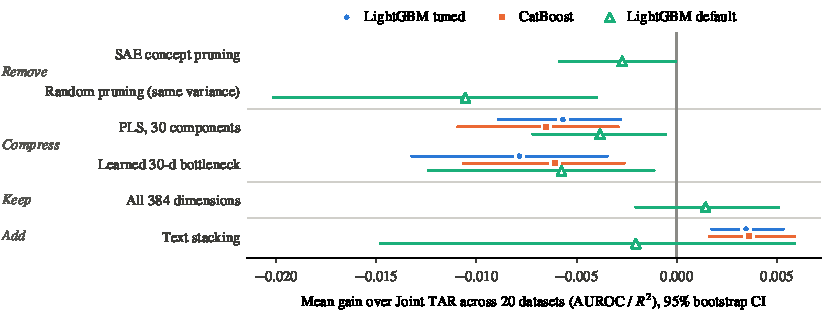
\includegraphics[width=\linewidth]{figures/overview.pdf}
\caption{Mean difference from Joint TAR over 20 datasets for every arm built on TAR's encoder, per learner (each
dataset: mean over 6 folds; bars: 95\% bootstrap interval over datasets). The wide default-LightGBM stacking interval
comes from Spotify genres (see text). Significance tests: Tables~\ref{tab:learners} and~\ref{tab:summary}.}
\label{fig:overview}
\end{figure}

\paragraph{Reweighting does not help.} PLS in place of PCA is worse than TAR with every learner ($-0.004$ to
$-0.007$; significant after correction with tuned LightGBM and CatBoost), and keeping all 384 dimensions is
indistinguishable from TAR ($+0.0014$, 9/20; Table~\ref{tab:summary}). This last arm tests the premise of
removal: if compressing TAR embeddings to 30 dimensions discarded much target-relevant information, keeping all 384
would win. It does not, so after fine-tuning there is little for a better compression to recover. Learning the
compression does not help either: the 30-unit bottleneck is worse than TAR with every learner ($-0.006$ to $-0.008$,
better on 3--6 datasets), almost entirely on binary and regression datasets (multiclass: $\le0.001$). A plausible
reason is that it keeps only what separates the training classes---for regression, the 20 bins---and discards finer
information that PCA on TAR's embedding retains. Late fusion helps on multiclass datasets
(6/7) but loses on all binary and regression datasets ($-0.018$ overall): averaging a table model and a text model
discards the interactions a joint learner can use.

\paragraph{Removing does not help, although its selection is meaningful.} Concept pruning on TAR is not better than
TAR ($-0.0027$, 8/20, $p=0.22$; in an earlier full run $-0.0035$, $p=0.006$). It removes about 70\% of the eligible
concepts and 38\% of the embedding variance (Table~\ref{tab:removal}), and the selection is meaningful: random removal
of the same variance is worse by $0.0078$ (16/20, $p<0.001$), and random removal of the same number of concepts, which
takes out 57\% of the variance, by $0.019$. 23\% of the dropped groups were never split on by either the concept or
its shadow, so ``removed'' partly means ``unused''. Sibling grouping rarely merged concepts, so redundant concepts
share gain inside the joint model rather than being tested as a unit. Making every decision on unseen rows does not
change the outcome: the cross-fitted variant (five datasets, Table~\ref{tab:xf}) ties TAR ($-0.0003$), choosing 0\%
where removal hurts and 75\% on two datasets where removal helped the inner encoders (trained on two thirds of the
rows) but not the final one.



% ------------------------------------------------------------------------------------------------------------
\section{Discussion, limitations and conclusion}

Our results suggest that after target-aware fine-tuning, little target-relevant information is lost in TAR's 30
components: keeping all 384 dimensions does not help, deleting concepts costs little but frees nothing, and replacing
PCA with PLS or a learned bottleneck makes results worse. Stacking helps for a different reason: its text model sees
all text columns together, before compression, and outputs the target directly, a summary the tree model cannot
easily assemble from 30 separate components per column. The gain is small ($\approx0.0035$) but appears
in every task type (datasets improved with tuned LightGBM and CatBoost: binary 3/3, 3/3; multiclass 6/7, 5/7;
regression 7/10, 9/10).

\emph{Limitations.} One encoder (E5-small) and one SAE size. Cross-fitting was run on five datasets only. Five default LightGBM multiclass
runs collapsed to chance level (four with stacking on Spotify, one held-out pruning run on Wine); the evidence points
to the learner, but we did not identify the mechanism. Single folds are sensitive to tiny numerical differences:
Recomputing the frozen embeddings on another GPU changed TAR + stacking on one fold by $0.012$, so our conclusions
rest on dataset-level tests.


\emph{Future work.} A stronger stacked model (e.g., the TAR-fine-tuned encoder with its head, out of fold),
other learners including tabular foundation models, and a diagnosis of the default-LightGBM collapse. Concept pruning
may be more useful on frozen encoders, in low-data settings, or as a diagnostic of which text concepts a model uses.


\emph{Conclusion.} On top of a fine-tuned encoder, target supervision helped when it added a text model's prediction,
not when it removed, reweighted, or re-learned the compression of the embedding. The code includes
\texttt{run\_csv.py}, which runs the method on any text--tabular CSV.




\small
\bibliographystyle{plainnat}
\bibliography{refs}

\normalsize
\appendix
\section{Additional results}\label{app:main}

\begin{table}[h]
\centering\small
\caption{Arms that change what follows TAR's encoder, per learner: mean difference from that learner's Joint TAR,
datasets improved (of 20), Wilcoxon $p$. Default-LightGBM Joint Frozen is in Table~\ref{tab:main} ($-0.017$, 1/20).}
\label{tab:learners}
\setlength{\tabcolsep}{3.5pt}\begin{tabular}{l}\toprule
\textit{[generated by make\_tables.py from the final run]}\\
\bottomrule\end{tabular}

\end{table}

\begin{table}[h]
\centering\small
\caption{Final run, default LightGBM: every arm vs.\ Joint TAR with the same fine-tuned encoder (per-dataset means
over 6 folds); $p$: Wilcoxon over datasets;   $p_{\text{Holm}}$: adjusted over all fourteen comparisons with TAR.}
\label{tab:summary}
\setlength{\tabcolsep}{3.5pt}\begin{tabular}{lccccc}
\toprule
Method & $\Delta$ vs.\ TAR & datasets won & folds won/lost & $p$ & $p_{\text{Holm}}$ \\
\midrule
TAR + text stacking & -0.0020 & 15/20 & 85/35 & 0.064 & 0.191 \\
TAR + PLS-30 (instead of PCA) & -0.0038 & 6/20 & 44/76 & 0.040 & 0.160 \\
TAR, learned 30-d bottleneck & -0.0058 & 6/20 & 39/81 & 0.015 & 0.092 \\
TAR, all 384 dims & +0.0014 & 9/20 & 63/57 & 0.729 & 0.729 \\
Late fusion (frozen text model) & -0.0181 & 6/20 & 39/81 & 0.030 & 0.148 \\
TAR + random pruning (variance-matched) & -0.0106 & 2/20 & 30/90 & $<$0.001 & $<$0.001 \\
TAR + concept pruning (ours) & -0.0027 & 8/20 & 48/72 & 0.216 & 0.432 \\
TAR + random pruning & -0.0217 & 1/20 & 19/101 & $<$0.001 & $<$0.001 \\
\bottomrule
\end{tabular}

\end{table}

\begin{table}[h]
\centering\small
\caption{What is removed from TAR embeddings, averaged over datasets, folds and text columns.}
\label{tab:removal}
\begin{tabular}{lccc}
\toprule
Removal & concepts removed & variance removed & removed groups never used \\
\midrule
Concept pruning (ours) & 70\% & 38\% & 23\% \\
Random, same number & 70\% & 57\% & -- \\
Random, same variance & 53\% & 39\% & -- \\
\bottomrule
\end{tabular}

\end{table}

\begin{table}[h]
\centering\small
\caption{Mean AUROC (classification) or $R^2$ (regression) over 6 folds, LightGBM. Best per row in bold.
$^\dagger$: fewer than 6 folds.}
\label{tab:main}
\begin{tabular}{lcccccc}
\toprule
Dataset & Frozen & TAR & TAR+prune & TAR+rand & PLS & Stack \\
\midrule
Fake job postings (bin) & 0.914 & 0.911 & 0.915 & 0.903 & 0.907 & \textbf{0.920} \\
Jigsaw toxicity (bin) & 0.819 & \textbf{0.933} & 0.929 & 0.880 & 0.864 & 0.864 \\
Kickstarter (bin) & 0.718 & \textbf{0.734} & 0.728 & 0.708 & 0.724 & 0.727 \\
DS salary (mul) & 0.798 & \textbf{0.807} & 0.803 & 0.797 & 0.793 & 0.806 \\
Michelin (mul) & 0.893 & \textbf{0.904} & 0.903 & 0.901 & 0.877 & 0.902 \\
Product sentiment (mul) & 0.874 & \textbf{0.890} & 0.887 & 0.889 & 0.846 & 0.879 \\
Spotify genres (mul) & 0.900 & 0.904 & \textbf{0.905} & 0.903 & 0.900 & 0.794 \\
US accidents (mul) & 0.970 & \textbf{0.978} & \textbf{0.978} & 0.975 & 0.970 & 0.973 \\
Wine reviews (mul) & 0.966 & \textbf{0.975} & \textbf{0.975} & 0.974 & 0.971 & 0.974 \\
Women's clothing (mul) & 0.898 & \textbf{0.906} & 0.904 & 0.903 & 0.896 & 0.902 \\
Baby product prices (reg) & 0.777 & 0.795 & 0.789 & 0.757 & \textbf{0.808} & 0.808 \\
Book prices (reg) & 0.496 & 0.514 & 0.499 & 0.469 & 0.501 & \textbf{0.521} \\
Book readability (reg) & 0.805 & \textbf{0.815} & 0.813 & 0.803 & 0.809 & 0.807 \\
Mercari (reg) & 0.414 & 0.439 & 0.433 & 0.409 & 0.437 & \textbf{0.445} \\
Montgomery salaries (reg) & 0.973 & 0.975 & 0.975 & \textbf{0.976} & 0.975 & 0.974 \\
Rotten Tomatoes (reg) & 0.494 & 0.506 & 0.500 & 0.474 & 0.480 & \textbf{0.509} \\
SCImago impact (reg) & 0.843 & \textbf{0.849} & 0.847 & 0.843 & 0.839 & 0.845 \\
Vancouver salaries (reg) & 0.734 & 0.765 & 0.768 & 0.756 & \textbf{0.769} & 0.766 \\
Video game sales (reg) & 0.368 & 0.379 & 0.355 & 0.255 & 0.369 & \textbf{0.384} \\
Zomato (reg) & 0.783 & 0.802 & 0.802 & 0.788 & 0.791 & \textbf{0.809} \\
\bottomrule
\end{tabular}

\end{table}

\begin{table}[h]
\centering\small
\caption{Final run, LightGBM: mean score per dataset for each TAR-based arm.}
\label{tab:finalmain}
\begin{tabular}{lccccccc}
\toprule
Dataset & TAR & +stack & +PLS & 384-d & Late & +prune & +rand(var) \\
\midrule
Fake job postings (bin) & 0.909 & 0.909 & 0.908 & \textbf{0.923} & 0.906 & 0.914 & 0.903 \\
Jigsaw toxicity (bin) & 0.932 & 0.932 & 0.924 & \textbf{0.936} & 0.881 & 0.929 & 0.927 \\
Kickstarter (bin) & \textbf{0.734} & 0.733 & 0.729 & 0.732 & 0.726 & 0.730 & 0.714 \\
DS salary (mul) & 0.807 & 0.809 & 0.796 & 0.800 & \textbf{0.827} & 0.803 & 0.804 \\
Michelin (mul) & 0.903 & 0.906 & 0.894 & 0.903 & \textbf{0.910} & 0.905 & 0.903 \\
Product sentiment (mul) & 0.890 & 0.896 & 0.878 & 0.889 & \textbf{0.910} & 0.890 & 0.889 \\
Spotify genres (mul) & 0.904 & 0.794 & 0.904 & 0.895 & \textbf{0.944} & 0.906 & 0.905 \\
US accidents (mul) & 0.978 & \textbf{0.979} & 0.977 & \textbf{0.980} & 0.969 & 0.979 & \textbf{0.979} \\
Wine reviews (mul) & 0.975 & 0.977 & 0.975 & 0.974 & \textbf{0.980} & 0.974 & 0.974 \\
Women's clothing (mul) & 0.905 & 0.905 & 0.902 & \textbf{0.907} & \textbf{0.907} & 0.905 & 0.905 \\
Baby product prices (reg) & 0.788 & \textbf{0.806} & 0.799 & 0.802 & 0.766 & 0.793 & 0.770 \\
Book prices (reg) & 0.512 & \textbf{0.516} & 0.499 & \textbf{0.516} & 0.465 & 0.499 & 0.484 \\
Book readability (reg) & 0.816 & \textbf{0.817} & 0.812 & 0.810 & 0.802 & 0.812 & 0.813 \\
Mercari (reg) & 0.442 & \textbf{0.453} & 0.439 & 0.441 & 0.422 & 0.431 & 0.419 \\
Montgomery salaries (reg) & 0.975 & 0.975 & \textbf{0.976} & 0.973 & 0.966 & 0.975 & 0.975 \\
Rotten Tomatoes (reg) & 0.504 & \textbf{0.516} & 0.482 & 0.510 & 0.496 & 0.494 & 0.493 \\
SCImago impact (reg) & 0.849 & \textbf{0.850} & 0.840 & 0.844 & 0.834 & 0.847 & 0.845 \\
Vancouver salaries (reg) & 0.767 & 0.766 & 0.774 & \textbf{0.781} & 0.649 & 0.770 & 0.764 \\
Video game sales (reg) & 0.384 & 0.374 & \textbf{0.386} & 0.370 & 0.297 & 0.361 & 0.300 \\
Zomato (reg) & 0.801 & 0.819 & 0.807 & \textbf{0.820} & 0.757 & 0.804 & 0.798 \\
\bottomrule
\end{tabular}

\end{table}

\begin{table}[h]
\centering\small
\caption{Nested cross-fitted removal amount (five datasets). Every decision is made on rows the judging encoder never
saw.}
\label{tab:xf}
\begin{tabular}{lccc}
\toprule
Dataset & TAR & TAR + cross-fitted pruning & chosen removal (per fold) \\
\midrule
Fake job postings & 0.912 & 0.911 & 75, 75, 75, 75, 75, 75\,\% \\
Jigsaw toxicity & 0.931 & 0.927 & 75, 75, 75, 75, 75, 75\,\% \\
Kickstarter & 0.734 & 0.734 & 0, 0, 0, 0, 0, 0\,\% \\
DS salary & 0.807 & 0.807 & 0, 0, 0, 0, 0, 0\,\% \\
Baby product prices & 0.789 & 0.794 & 50, 50, 10, 25, 0, 25\,\% \\
\bottomrule
\end{tabular}

\end{table}



\end{document}
